\documentclass{standalone} % Use standalone for easy compilation
\usepackage{tikz}
\usetikzlibrary{
    shapes.geometric, % For shapes like diamond, trapezium, cylinder
    arrows.meta,      % For arrow tip styles
    positioning,      % For relative positioning (below=of ...)
    fit,              % To fit nodes around others
    backgrounds,      % To draw behind nodes
    shadows           % For subtle shadows
}

\begin{document}

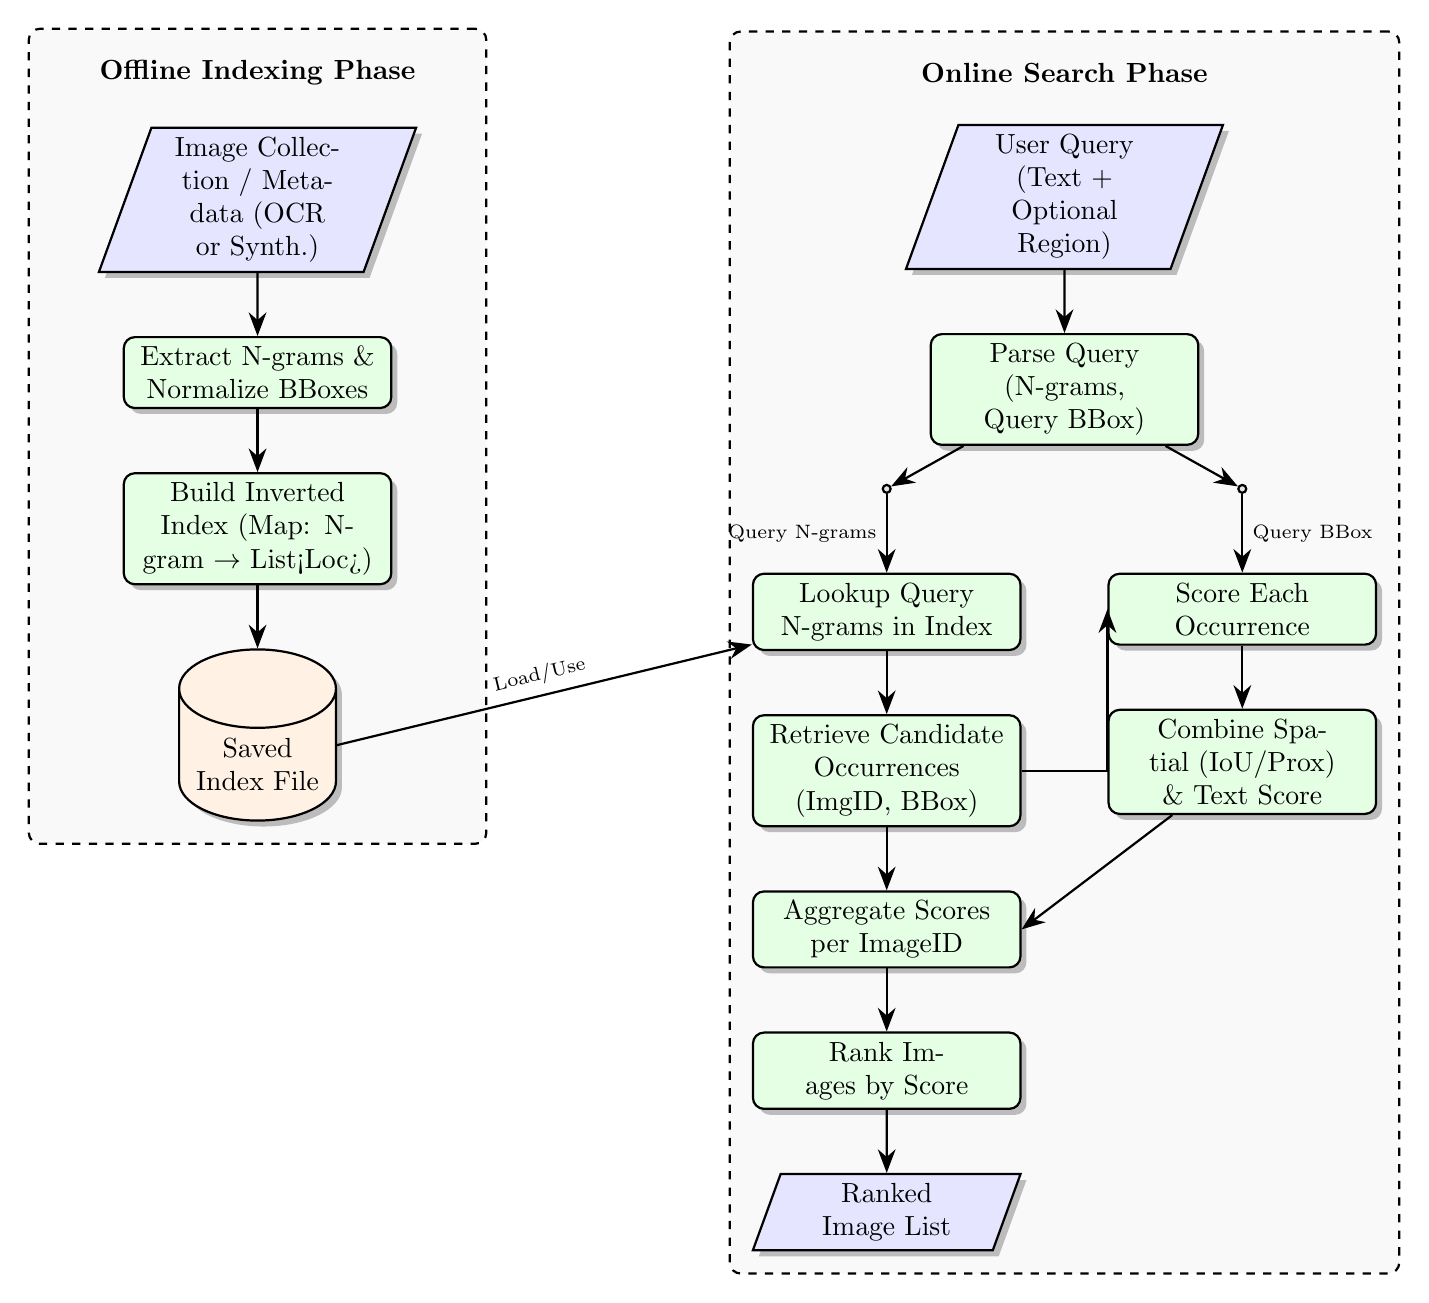
\begin{tikzpicture}[
    node distance=8mm and 12mm, % Control vertical and horizontal spacing
    % Define styles
    input/.style={trapezium, trapezium left angle=70, trapezium right angle=110, draw, thick, fill=blue!10, drop shadow, minimum height=2.5em, text centered, text width=7em}, % Input/Output data
    process/.style={rectangle, draw, thick, fill=green!10, rounded corners, drop shadow, minimum height=2.5em, text centered, text width=9em}, % Processing step
    storage/.style={cylinder, shape border rotate=90, draw, thick, fill=orange!10, drop shadow, minimum height=3em, aspect=0.5, text centered, text width=5em}, % Index storage
    connector/.style={circle, draw, thick, fill=gray!20, minimum size=1mm, inner sep=0pt}, % Small connector nodes for cleaner lines
    arrow/.style={thick, -{Stealth[length=3mm]}}, % Arrow style
    phasebox/.style={rectangle, draw, thick, dashed, rounded corners, inner sep=8pt, fill=gray!5} % Box around phases
]

% ----- OFFLINE INDEXING PHASE -----
\node (offline_label) [text width=5cm, align=center, font=\bfseries] {Offline Indexing Phase};
\node (in_data)     [input, below=4mm of offline_label] {Image Collection / Metadata (OCR or Synth.)};
\node (proc_extract)[process, below=of in_data] {Extract N-grams \& Normalize BBoxes};
\node (proc_build)  [process, below=of proc_extract] {Build Inverted Index (Map: N-gram $\to$ List<Loc>)};
\node (idx_store)   [storage, below=of proc_build] {Saved Index File};

% Draw arrows for offline phase
\draw [arrow] (in_data) -- (proc_extract);
\draw [arrow] (proc_extract) -- (proc_build);
\draw [arrow] (proc_build) -- (idx_store);


% ----- ONLINE SEARCH PHASE -----
\node (online_label) [text width=5cm, align=center, font=\bfseries, right=50mm of offline_label] {Online Search Phase};
\node (in_query)    [input, below=4mm of online_label] {User Query (Text + Optional Region)};
\node (proc_parse)  [process, below=of in_query] {Parse Query (N-grams, Query BBox)};
\node (c1)          [connector, below left=5mm and 5mm of proc_parse] {}; % Connector
\node (c2)          [connector, below right=5mm and 5mm of proc_parse] {}; % Connector
\node (proc_lookup) [process, below=10mm of c1] {Lookup Query N-grams in Index};
\node (proc_retrieve)[process, below=of proc_lookup] {Retrieve Candidate Occurrences (ImgID, BBox)};
\node (proc_score)  [process, below=10mm of c2] {Score Each Occurrence};
\node (proc_combine)[process, below=of proc_score] {Combine Spatial (IoU/Prox) \& Text Score};
\node (proc_agg)    [process, below=of proc_retrieve] {Aggregate Scores per ImageID};
\node (proc_rank)   [process, below=of proc_agg] {Rank Images by Score};
\node (out_results) [input, below=of proc_rank] {Ranked Image List};


% Draw arrows for online phase
\draw [arrow] (in_query) -- (proc_parse);
\draw [arrow] (proc_parse) -- (c1);
\draw [arrow] (proc_parse) -- (c2);
\draw [arrow] (c1) -- node[left, font=\scriptsize] {Query N-grams} (proc_lookup);
\draw [arrow] (c2) -- node[right, font=\scriptsize] {Query BBox} (proc_score);
% Arrow from Index Store to Lookup
\draw [arrow] (idx_store) -- node[above, font=\scriptsize, sloped] {Load/Use} (proc_lookup);
\draw [arrow] (proc_lookup) -- (proc_retrieve);
\draw [arrow] (proc_retrieve) -- (proc_agg);
% Connect retrieve candidates to scoring
\draw [arrow] (proc_retrieve.east) -| (proc_score.west);
\draw [arrow] (proc_score) -- (proc_combine);
\draw [arrow] (proc_combine) -- (proc_agg.east); % Feed combined score to aggregation
\draw [arrow] (proc_agg) -- (proc_rank);
\draw [arrow] (proc_rank) -- (out_results);


% ----- FIT PHASE BOXES (using background layer) -----
\begin{pgfonlayer}{background}
    \node [phasebox, fit=(offline_label) (in_data) (proc_extract) (proc_build) (idx_store)] {};
    \node [phasebox, fit=(online_label) (in_query) (proc_parse) (proc_lookup) (proc_retrieve) (proc_score) (proc_combine) (proc_agg) (proc_rank) (out_results) (c1) (c2)] {};
\end{pgfonlayer}

\end{tikzpicture}

\end{document}
